\section{Testing of the Project}
\label{sec:testing}

\subsection{Functional Testing}
In this section, each of the functional requirements laid out in section \ref{sec:funcs} have been evaluated and tested, to ensure that the system meets them. Due to these tests coming directly from the requirements, it was easy to determine if each test was successful or not, based on whether or not the feature had been included. In cases where the test is marked as ``passed'', a screen shot of evidence has been provided. This testing was only interested in whether or not specific features were present, and the inner workings of these features was irrelevant, for this reason, these can be considered black box tests\cite{beizer1995black} (testing where only the input and output can be observed).\ \\
\ \\
\noindent 
\begin{tabular}{p{1.2cm}|p{5.85cm}|p{1.1cm}|p{5.85cm}}
	\hline	
	\textbf{FR\#} & \textbf{Test} & \textbf{Result} & \textbf{Proof} \\
	\hline
	1.    & Users can search by geographical region & Passed &
 \raisebox{-\totalheight}{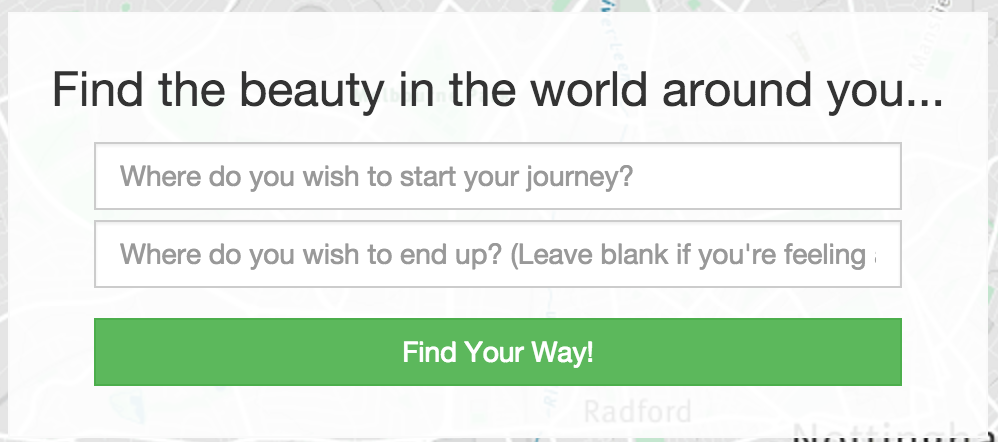
\includegraphics[width=0.4\textwidth]{images/testing/fr1.png}}\\
	\hline
	2.    & Users can contribute routes & Passed & See 2.1 and 2.2\\
	\hline
	2.1. & The creator of a route (only) can modify it & Passed &  \raisebox{-\totalheight}{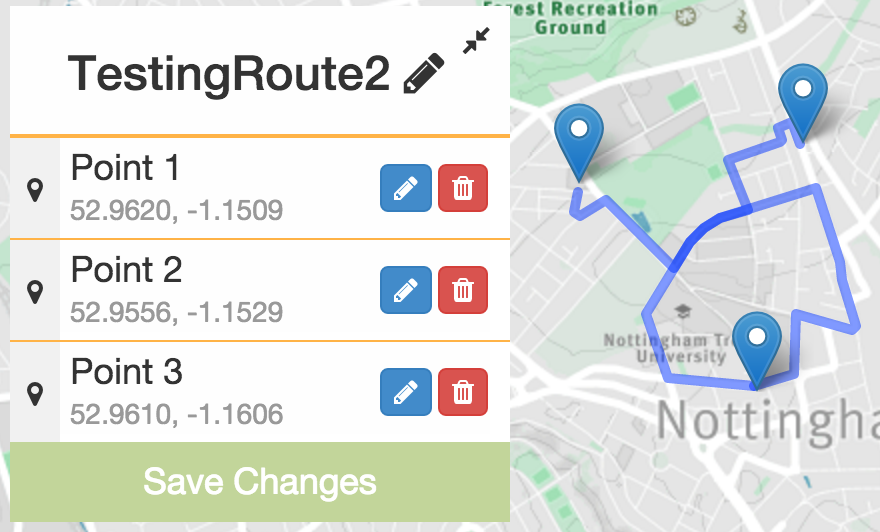
\includegraphics[width=0.4\textwidth]{images/testing/fr2-1.png}}\\
	\hline
	2.2  & Users can make their routes private & Passed & \raisebox{-\totalheight}{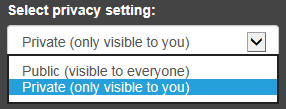
\includegraphics[width=0.4\textwidth]{images/testing/fr2-2.png}}\\
	\hline
	3.    & Users can interact socially with routes & Passed & See 3.1, 3.2 and 3.3\\
	\hline
	3.1. & Users can comment on routes & Passed & \raisebox{-\totalheight}{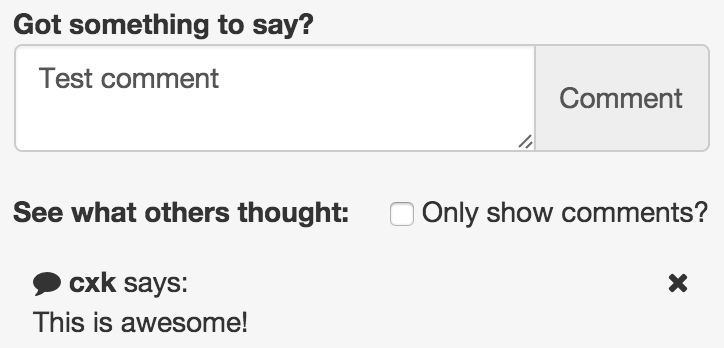
\includegraphics[width=0.4\textwidth]{images/testing/fr3-1.png}}\\
	\hline
	3.2. & Users can recommend routes similar to the current route & Passed & \raisebox{-\totalheight}{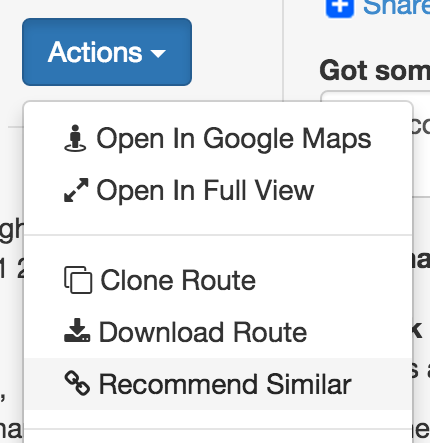
\includegraphics[width=0.175\textwidth]{images/testing/fr3-2.png}}\\
	\hline
\end{tabular}
\vspace{-10mm}

\newpage 
\noindent
\begin{tabular}{p{1.2cm}|p{5.85cm}|p{1.1cm}|p{5.85cm}}
	\hline	
	\textbf{FR\#} & \textbf{Test} & \textbf{Result} & \textbf{Proof} \\
	\hline
	3.3. & Users can share routes externally & Passed & \raisebox{-\totalheight}{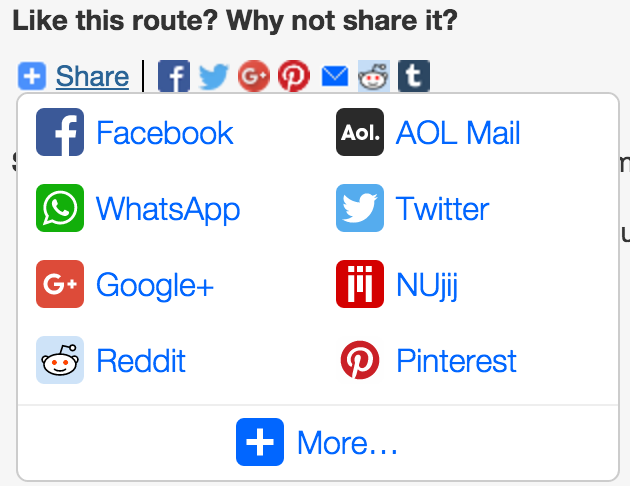
\includegraphics[width=0.35\textwidth]{images/testing/fr3-3.png}}\\
	\hline
	4.    & Users can create accounts & Passed & \raisebox{-\totalheight}{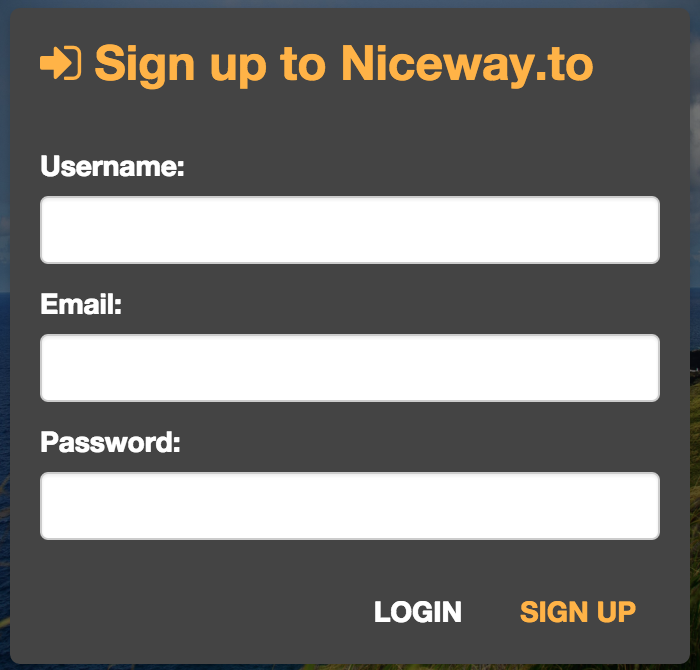
\includegraphics[width=0.35\textwidth]{images/testing/fr4.png}}\\
	\hline
	5.    & There are administrative users & Passed & \raisebox{-\totalheight}{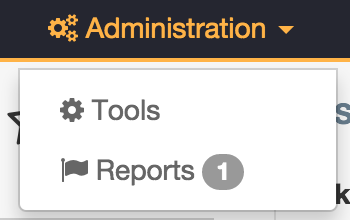
\includegraphics[width=0.3\textwidth]{images/testing/fr5.png}}\\
	\hline
	5.1. & Administrators can delete users & Passed & \raisebox{-\totalheight}{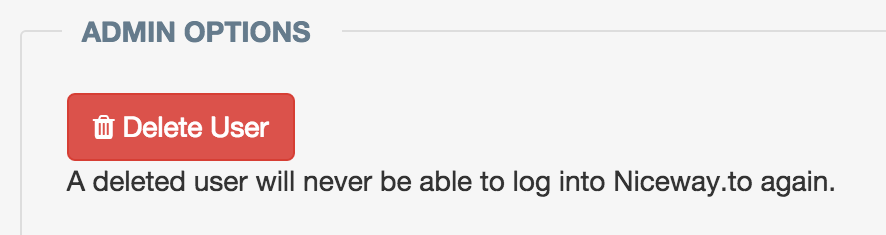
\includegraphics[width=0.4\textwidth]{images/testing/fr5-1.png}}\\
	\hline
	5.2. & Administrators can update users  & Passed & \raisebox{-\totalheight}{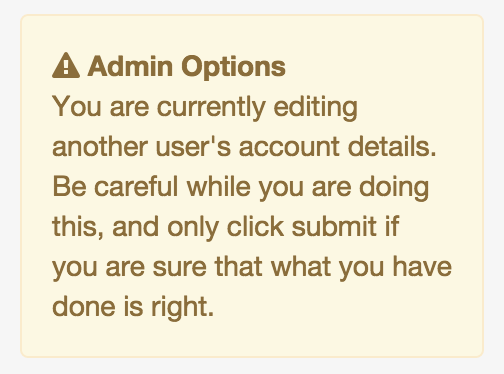
\includegraphics[width=0.4\textwidth]{images/testing/fr5-2.png}}\\
	\hline
	5.3. & Administrators can create users & Passed & \raisebox{-\totalheight}{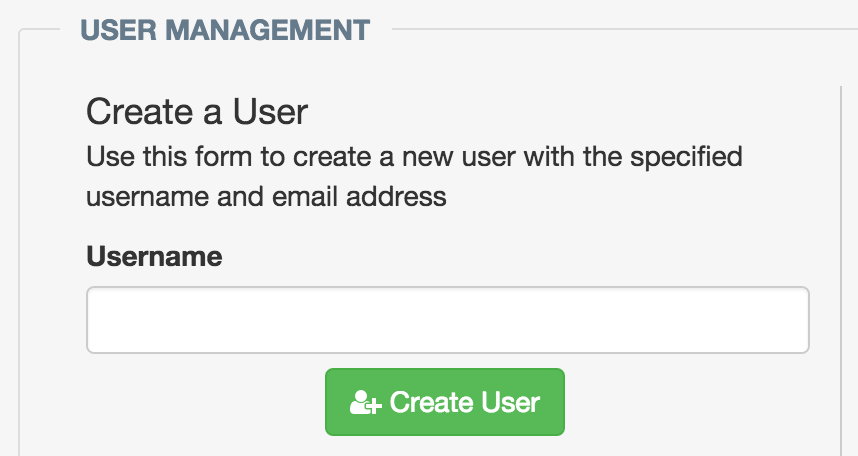
\includegraphics[width=0.4\textwidth]{images/testing/fr5-3.png}}\\
	\hline
\end{tabular}

\newpage 
\noindent 
\begin{tabular}{p{1.2cm}|p{5.85cm}|p{1.1cm}|p{5.85cm}}
	\hline	
	\textbf{FR\#} & \textbf{Test} & \textbf{Result} & \textbf{Proof} \\
	\hline
	5.4. & Administrators can delete routes & Passed & \raisebox{-\totalheight}{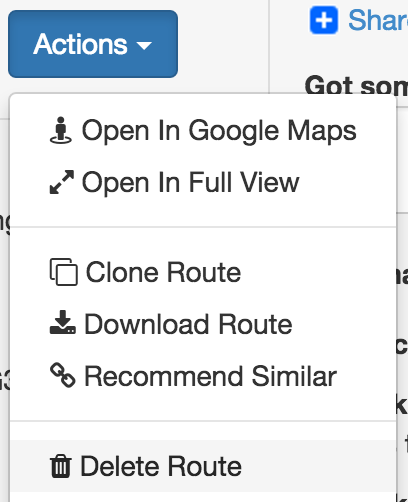
\includegraphics[width=0.25\textwidth]{images/testing/fr5-4.png}}\\
	\hline
	5.5. & Administrators can delete user comments made on routes & Passed & \raisebox{-\totalheight}{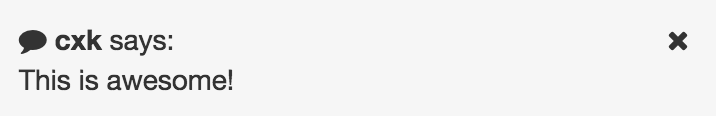
\includegraphics[width=0.4\textwidth]{images/testing/fr5-5.png}}\\
	\hline
	5.6. & Administrators can post messages that will be displayed on every page   & Passed & \raisebox{-\totalheight}{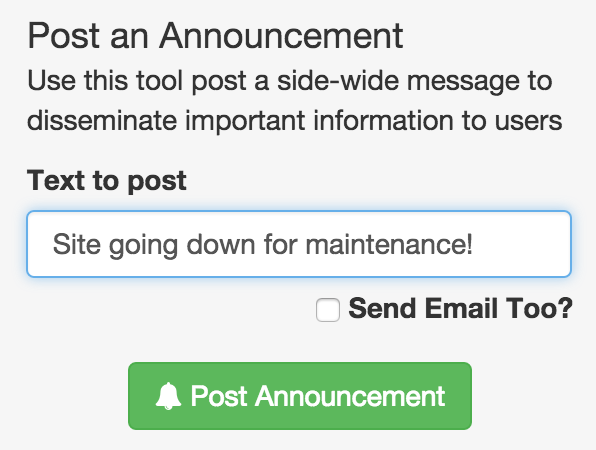
\includegraphics[width=0.4\textwidth]{images/testing/fr5-6.png}}\\
	\hline
	5.7. & Administrators can make backups & Passed & \raisebox{-\totalheight}{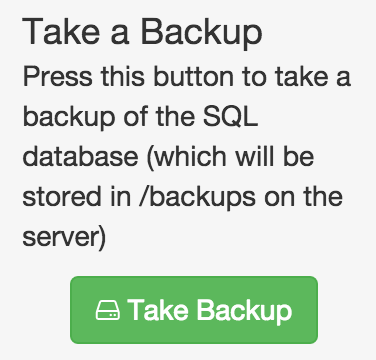
\includegraphics[width=0.3\textwidth]{images/testing/fr5-7.png}}\\
	\hline
	5.8. & Administrators can close and deauthorize active sessions & Passed & \raisebox{-\totalheight}{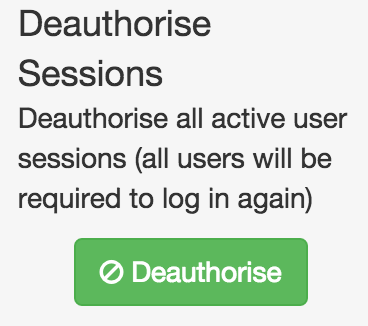
\includegraphics[width=0.3\textwidth]{images/testing/fr5-8.png}}\\
	\hline
	5.9. & Administrators can lock the site & Passed & \raisebox{-\totalheight}{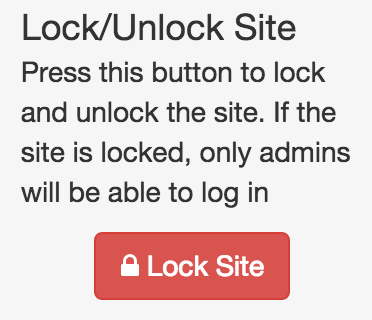
\includegraphics[width=0.3\textwidth]{images/testing/fr5-9.png}}\\
	\hline
\end{tabular}

\newpage 
\noindent 
\begin{tabular}{p{1.2cm}|p{5.85cm}|p{1.1cm}|p{5.85cm}}
	\hline	
	6.    & Users can export/download their routes & Passed & \raisebox{-\totalheight}{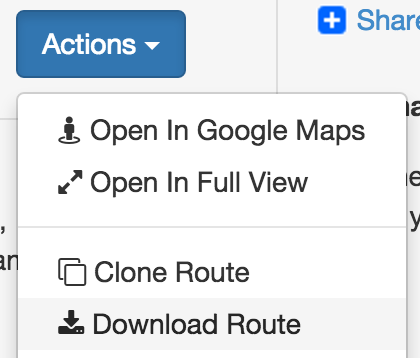
\includegraphics[width=0.3\textwidth]{images/testing/fr6.png}}\\
	\hline
	7.    & Users can make a copy of another user's route & Passed & \raisebox{-\totalheight}{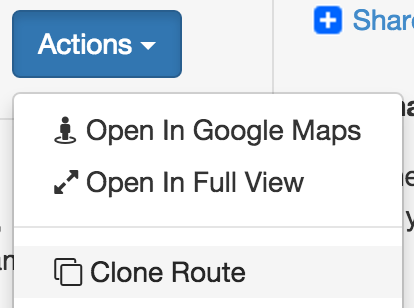
\includegraphics[width=0.3\textwidth]{images/testing/fr7.png}}\\
	\hline
	8.    & There is a route creation/editing component & Passed & \raisebox{-\totalheight}{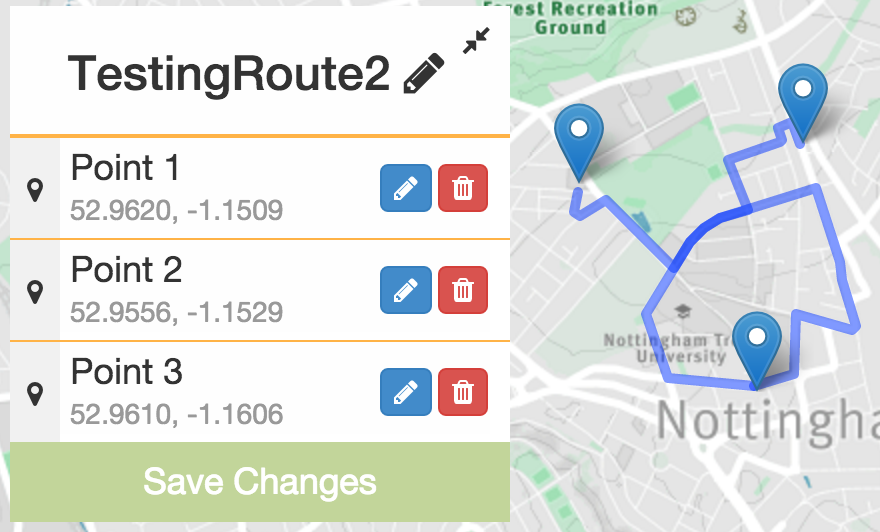
\includegraphics[width=0.4\textwidth]{images/testing/fr8.png}}\\
	\hline
	9.    & Users can log into their account & Passed & \raisebox{-\totalheight}{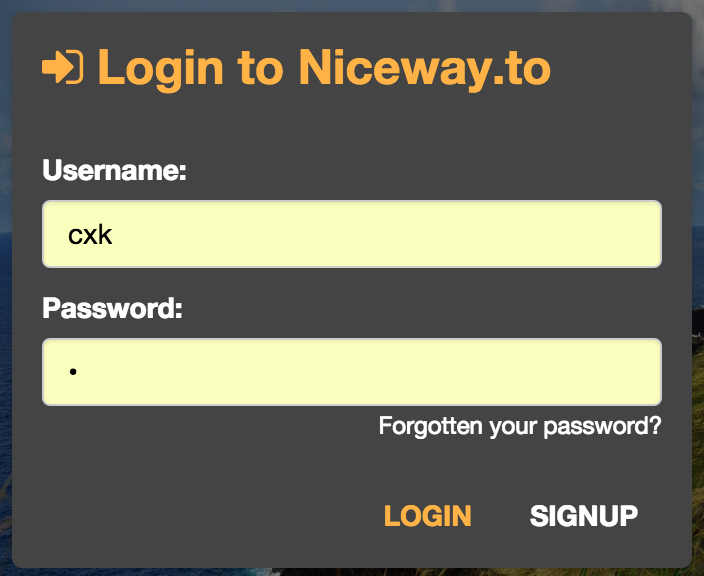
\includegraphics[width=0.3\textwidth]{images/testing/fr9.png}}\\
	\hline
	9.1. & Users can edit their personal information & Passed & \raisebox{-\totalheight}{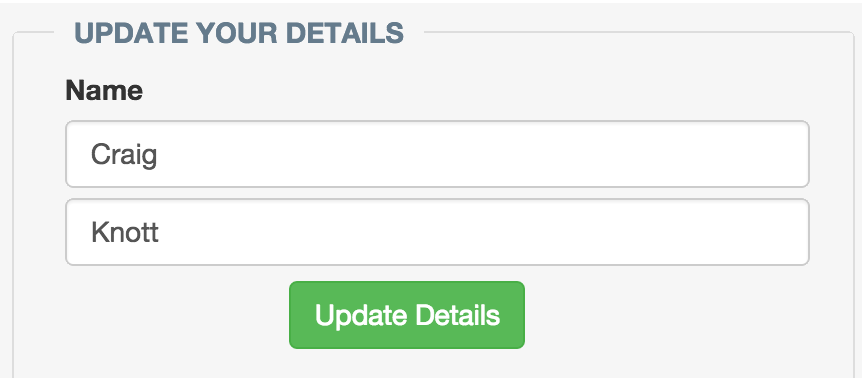
\includegraphics[width=0.4\textwidth]{images/testing/fr9-1.png}}\\
	\hline
	9.2. & Users can access and edit their routes & Passed &\raisebox{-\totalheight}{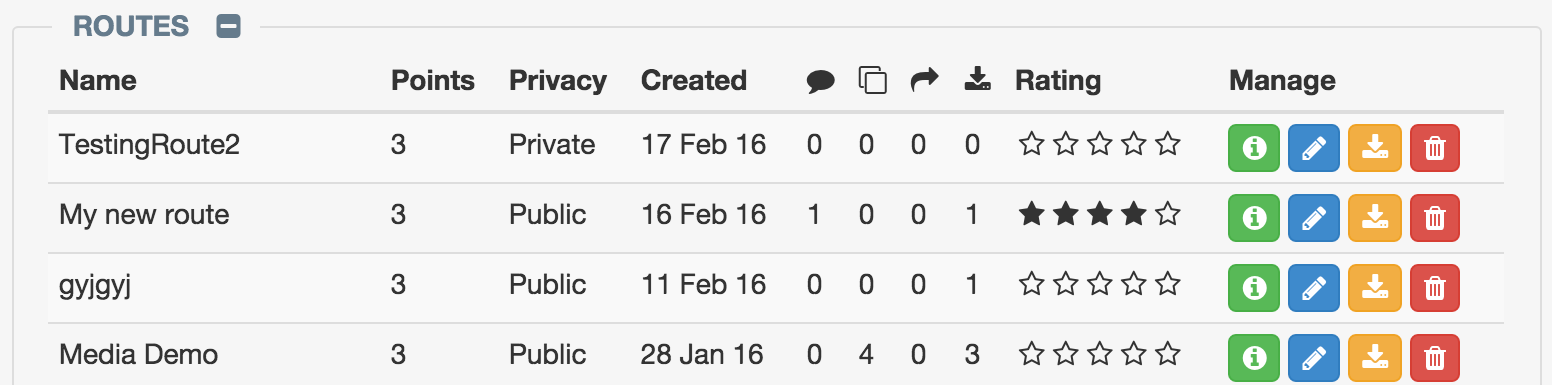
\includegraphics[width=0.4\textwidth]{images/testing/fr9-2.png}} \\
	\hline
\end{tabular}

\newpage 
\subsection{Non-Functional Testing}
In this section, each of the non-functional requirements defined in section \ref{sec:nfuncs} have been evaluated, and steps taken to ensure they were adhered to have been listed.


\paragraph{Accessibility}\ \\
To ensure the service was accessible for the largest number of people, it was developed as a fully responsive web application, rather than a native mobile application. This meant that any users with an Internet connection could access the site, regardless of device. As a website, the project relied on the server to allow users to continually access it, for which there were two main concerns: the domain expiring, and the server going down. The solution to the first of these was setting up reminders to renew the domain when necessary, and the solution to the second would be to set up backup servers (although that was not within the scope of this project).

\paragraph{Usability and Operability}\ \\
To ensure that all users, regardless of skill level, could use the system effectively, it was designed to be as leading and simple as possible. This meant having large buttons to draw the eye to certain key tasks, decorating pages with well known icons (so users could easily determine what the functionality of each item should be), ensuring that simple language was used throughout, and the interface free of clutter, or at least presented in an organised way. As mentioned above, the application was developed as a fully responsive web application, utilising Twitter's Bootstrap framework, therefore allowing users of any device to access the website.

\paragraph{Maintainability \& Documentation}\ \\
This requirement was partially met simply through the use of the Zend Framework, which enforces a Model View Controller design pattern. This meant that it was already modular, and the form was separate from the function. This, along with the extensive documentation and standards that have been produced for the Zend Framework, meant that understanding different segments of the code is simple.\ \\
\ \\
In addition, every function and class has been commented with PHPDoc (or a JavaScript equivalent for the JavaScript code), and therefore functionality of each individual block of code is immediately obvious, and an external developer should be able to understand what each block does, and how to use it.

\paragraph{Quality}\ \\
To ensure the software was of the highest quality, the standards defined above were strictly adhered to, including the use of Zend standards, and extensive commenting of code. To ensure that the quality of the product was equally as high, all new functionality was tested vigorously to ensure that it was free of bugs, and that it did not introduce bugs to other parts of the software. Further to this, the RITE method for identifying usability issues (which is discussed further in section \ref{sec:rite}) was employed with 15 individuals, to identify any potential problems with the interface. 

\paragraph{Resource Requirements and Constraints}\ \\
To ensure that the system was not a burden on the user's hardware, it was designed to do as much computation and calculation on the server side as possible. This meant that the server was responsible for doing the majority of the work, and the client would be spared. Even after page loads and the user did some interaction, an AJAX call would be made, which would get results, do computation, and then only have to quickly update the DOM of the page to reflect these changes.\ \\
\ \\
The downloadable files (of routes) produced by the website were saved in JSON format, so that the signal-to-noise ratio (the amount of data used to describe the data itself) was kept to a minimum, meaning the size of the file was reduced. Even extremely large routes saved in this format would have minuscule file sizes (as a test, a route with 50 points was created, which only had a file size of 6KB).\ \\
\ \\
The final consideration was the amount of data being sent to the user, and keeping this to a minimum. For this reason, all libraries in the project were minified (both JavaScript and CSS), to reduce the total data expenditure. After the project is released fully, the JavaScript and CSS of each page can also be minified to further reduce the size of each web page. 

\paragraph{Cross Platform Compatibility}\ \\
Due to the project being a website, it was inherently cross-platform compatible, because it is rendered within a web browser rather than a specific application or operating system. However, there are many intricacies within each web browser, and therefore it was necessary to test the core functionality of the application in each of the main web browsers: Google Chrome, Internet Explorer, Mozilla Firefox, and Apple Safari. Despite some graphical differences due to how each browser renders page differently, the core functionality worked across each of these browsers (which served to increase the size of the user base that could be targeted).

\paragraph{Security}\ \\
As users were signing up for accounts for the system, they could provide some personally identifiable information. For this reason, both access to the web server, and access to the database running on the server required a correct user name and password. In addition to this, the passwords for all users were stored as an encrypted MD5 hash, to ensure that no member of the Niceway.to team could access a user's account unlawfully. \ \\
\ \\
Some information that users can enter is also displayed on their profile page. For this reason, a disclaimer is included on the settings page, so that users can see what pieces of information will be publicly visible. This included: user name, age, length of membership, public routes, and location, but explicitly \textit{not} email address. This meant that the user had the freedom to choose which pieces of information they shared, and which they would not.

\paragraph{Disaster Recovery}\ \\
There were several methods employed to aid in disaster prevention and recovery for Niceway.to. Other than having access to the server, and the ability to use the UNIX system to run whatever commands were necessary, the administrators of the site also had several tools available within the application that they could use. The first of these was the ability to take backups of the site, which would save a copy of a mysqldump of the database to a directory on the web server, allowing the site to be restored to a previous state if necessary. The second tool was the ability to de-authorize all active sessions, meaning that any users would be required to log in again, before continuing to use the site (useful if hackers had infiltrated user accounts). The final tool was the ability to lock the site, which would prevent any users that were not administrative users from logging into the site, instead presenting them with a message informing them that Niceway.to was down for maintenance.

\newpage 
\subsection{User Feedback Testing}
\label{sec:rite}
Usability testing is the process of getting actual users to use the system, with these users performing a set of tasks whilst being observed. The time taken to complete the various tasks, and any comments or criticisms the user had were recorded, as well as any bugs the user encountered. The purpose of these tests was to discover usability problems in the interface, and what could be made simpler.\ \\
\ \\
For the tests a sample of 15 users were selected, with a skill level ranging from low, to very high, and ages ranging from 21 to 46. The reason for this broad range was that users of different skill levels, and different ages, use and understand computers differently, and therefore what is considered intuitive for one user is not necessarily considered the same by others. This meant that the number of usability issues and simplifications that could be identified was greatly increased. The five tasks that the users were expected to complete are given below, and a full list of instruction can be found in appendix \ref{sec:utis}.

\begin{enumerate}
	\item Search for a route, and view its details
	\item Create an account for the system
	\item Comment, rate and download a route 
	\item Create a route
	\item Navigate back to their route, and make edits
\end{enumerate}
\noindent 
These five tasks represented the five core tasks that users of Niceway.to would be expected to engage in on a regular basis (except signing up, which would only occur once, but was a barrier for entry so it was important it was short and simple). This meant it was vital that they were easy to understand, and easy to complete by users of all skills levels. It was for this reason that the instructions for the tests were as vague as possible, as not to lead the users to the correct answers. Some of these tasks were purposefully extremely simple and short, so that users could really focus on the specific areas of the system, and therefore identify more issues.\ \\
\ \\
The RITE method (Rapid Iterative Testing and Evaluation) was employed during the usability tests to quickly iterate on user feedback to fix issues within the system. This meant that, after each user completed the set of tasks, their feedback would be implemented, and any bugs they discovered would be fixed before the start of the next test. Each participant would therefore be looking at a slightly different product, and they would all be able to identify unique issues instead of all being focused on the same issues.

\begin{figure}[!ht]
	\begin{center}
		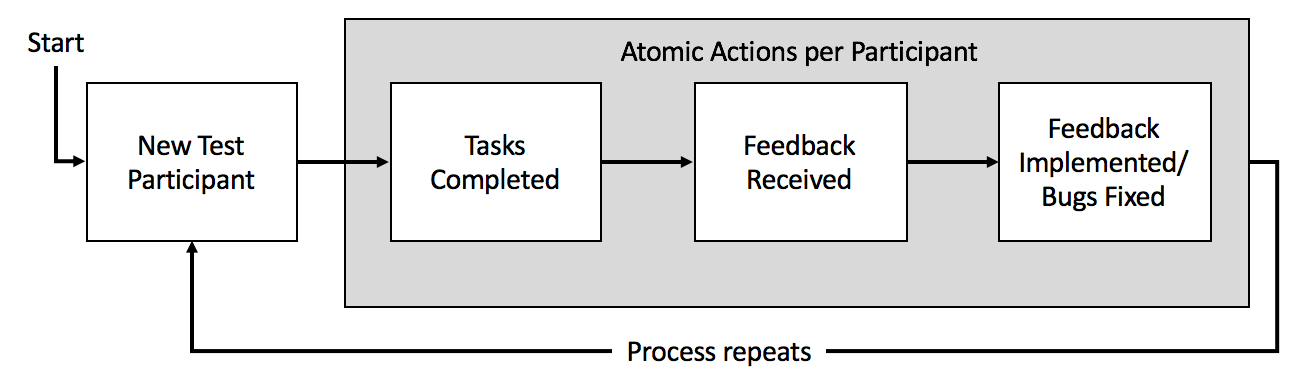
\includegraphics[width=0.9125\textwidth]{images/testing/rite.png}
	\end{center}
	\vspace{-6mm}
	\caption{The employed RITE method life cycle}	
	\vspace{-6mm}
\end{figure}

\newpage
\noindent
The time taken for each participants to complete the tasks can be found in appendix \ref{sec:trfut}, with a summary presented below, and an discussion of these results forthwith.

\begin{figure}[!ht]
	\vspace{-1mm}
	\begin{center}
		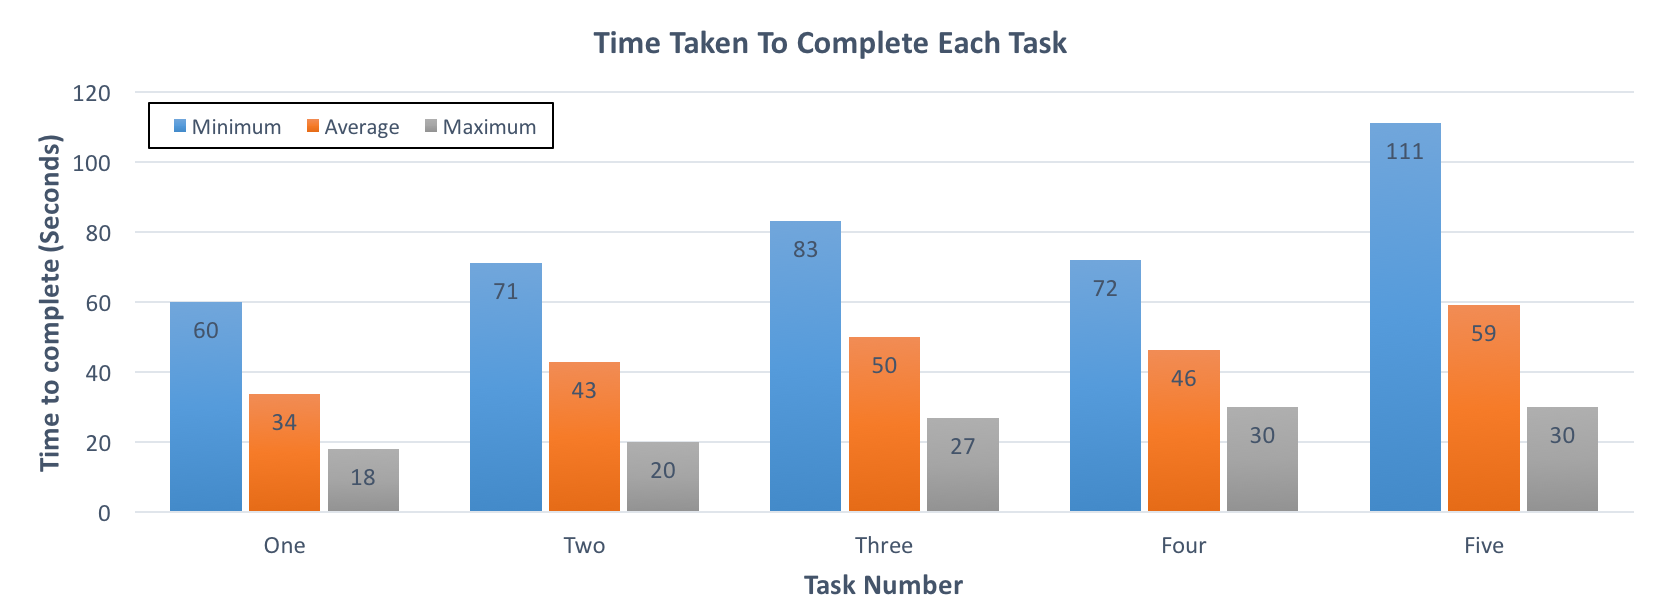
\includegraphics[width=0.9\textwidth]{images/testing/results.png}
	\end{center}
	\vspace{-7mm}
	\caption{Summarised results from user testing}	
	\vspace{-2mm}
\end{figure}

\noindent
From these results it would not be far-fetched to claimed that each of these tasks were simple to achieve. They could all be completed in under two minutes by users of all skills levels, with an average completion time of just under a minute. Some expert users could even complete the tasks in under thirty seconds, which is promising, and is a figure that many users would eventually be able to replicate, as their usage of the site increased. A brief analysis of each of the tasks is given below.

\paragraph{Task One - Searching for Routes}\ \\
This task was completed fastest of them all, which in part is due to users starting on the page they needed to use, but also that the functionality was easy to locate. This was because of the large search box in the middle of the page, which was eye catching and intuitive for users to understand. The main limiting factor in this test was not the software, but rather how quickly the user could type the search terms, which was the cause for the differing times. On the search results page, most users were almost instantly able to find the link to the details page, and complete the test unhindered. One user attempted to click on the title of the route, which he believed to be the ``more intuitive thing to do'', and thus this functionality was added after that user completed their testing.

\paragraph{Task Two - Creating an Account}\ \\
Creating an account required the user to enter a user name, their email, and a password. This was therefore an extremely simple task, that most users performed with little hindrance. The main factors that drove the time up for this task were the waiting for the confirmation email (which varied based on the participants Internet connection speed), and errors in the form. The main error being users entering passwords that were too short (less than six characters), and their accounts being rejected as a result. This meant that users has to completed this step again, and spend some time trying to understand the problem. None of these, however, were points of discussion, as most users accepted this as standard, and didn't feel like it was a usability problem.\ \\
\ \\
One issue that was not addressed in this process was what happens when a user attempted to sign up with a user name that already exists in the system. This is because there were so few accounts created, that the odds of two users picking the same were minuscule. If a user did happen to pick the same user name as someone else, it would likely result in a highly inflated time for this task, because the user would then be required to think of another unique user name, which can be difficult, as most users tend to use the same one for most websites. 

\paragraph{Task Three - Interaction with a Route}\ \\
The third task was used to determine how easy it was to experience the social elements of the system, which was an extremely important part of the system in regards to building a community around the website. In this task, users were required to search for a route and open it (building on knowledge they acquired in the first task), then perform three social interactions: commenting on the route, giving the route a rating, and downloading the route. Of these three, the only one that users struggled with was the downloading of the route, as many users could not find this option. It was clear that most users expected the download button to be somewhere in plain site, which was due to them being unaware of the other interactions they could have with the route, and thus assumed the download functionality be available just like commenting on routing. After the users discovered the action button, they quickly found the download feature, as well as a host of other features, which would then be able to use next time they were on the site.
\ \\
\paragraph{Task Four - Creating a Route}\ \\
It is worth pointing out that, despite the results for this test being very positive, there are not indicative of how a real user would use the route creation page. In the tests, users were simply asked to construct a route with three points, and save it. A real user would spend much longer in positioning these points, ensuring the route between them was good, and adding rich content, like titles, descriptions and media to the points. In the tests, most users clicked on three places at random, and hit the save button. It may have been beneficial to enforce the users to look for specific locations, which would have better reflected real users.\ \\
\ \\
Regardless of this, a lot of useful feedback was gathered from these tests. The most prominent (which could have easily been missed as a result of the format of the test), was the difficultly of navigating large portions of the map at once. This was only discovered when one user that was not local to Nottingham, decided to create a route started at his house in Guildford. This required him to scroll the map for a considerable time to find this location. As a result of this feedback, the ability to search for specific locations, and centre the map on them, was added to the route creation page. This meant that users could search for a location and instantly jump to it, which  was useful for when they wanted to create a route that started far away from their initial location.
\ \\
\paragraph{Task Five - Editing your Route}\ \\
The fifth task was the task that, on average, took the longest to complete, and had the greatest range of results (with a difference of 81 seconds between the fastest and slowest times). This is most probably caused by the users requiring some level of intuition to finish the task. In two of the previous tasks, the user was asked to use the search functionality, but in this task they were told to specifically avoid it. This meant the user needed to think about the system and utilise tools they had already used (the navigation bar), but apply them to a new problem - finding where their routes were saved.\ \\
\ \\
After users determined that their routes were stored in the ``My Profile'' area of the site, locating the ability to edit them was very simple. The synonimity of a pencil icon, and the ability to edit is very strong, and many users (after locating the specific route), jumped to the edit page very shortly after. Perhaps changing the testing instructions to use the word ``modify'' or ``change'', rather than ``edit'', would have had an impact here.

\newpage
\noindent
An interesting thing to point out in task five, which was a merit of the RITE method, was how the editing of titles changed as a result of the tests conducted. One of the first users commented that having to click ``Save'' before being able to change the title was cumbersome. He suggested putting an edit icon next to the title, and allowing users to change this value - which would be more intuitive. This feedback was then implemented and it was observed that every single participant utilised this new feature, and thus sped up the time it took to complete that particular task

\paragraph{Issues Identified}\ \\
Some of the main issues that were identified during the usability tests, and were then resolved in between testing stages, have been listed below. The advantage of resolving these issues in between tests is that subsequent participants were able to detect unique and novel issues, rather than each user identifying the same set of issues.
\ \\
\ \\
\noindent 
\begin{tabular}{p{1.5cm}|p{6.25cm}|p{6.25cm}}
	\hline 
	\textbf{Page} & \textbf{Comments Made} & \textbf{Resolution} \\
	\hline 
	\lbrcell{Landing} & ``Why can't I press enter to search?'' & Allowed users to press the return key to submit their search results on the landing page.\\
	\hline
	\lbrcell{Landing} & ``I accidentally searched without a starting point and got loads of errors'' & Prevented users from submitting their search if no start point was provided.\\
	\hline	
	Listing & ``I thought that clicking on the title would have been the more intuitive thing to do'' & Allowed users to click on the title of a search result to view full details\\
	\hline	
	Listing & ``After I clicked on a route, I clicked the back button and there was an error about having to resubmit a form and I couldn't get my original search results back'' & Changed form submission mechanics so users could press the back button to access their original search results\\
		\hline
		\lbrcell{Listing} & ``Some of the route were really long and didn't fit in the map box'' & The maximum zoom limit for routes on the listing and detail page was removed\\
	\hline		
	Creation & ``It was strange that I couldn't rename my route unless I opened the save popup, especially considering how the title is displayed on the page already'' & An edit icon was added to the title, which users could click on to modify their route title, without having to open the save dialogue.\\
	\hline
	Creation & ``I had to scroll and pan for a very long time to get the map to centre over my house in Guildford, because it started in Nottingham'' & Added a search box on the route creation page that would take the entered location and centre the map on this point\\ 
	\hline
	Creation & ``I was worried that clicking `Save Route' would create a new, duplicate, route'' & Changed button to read `Save Changes' instead, when on the edit page. \\
	\hline
	Creation & ``I accidentally deleted one of my points, and the `Loading Map' thing stayed forever'' & Modified behaviour of the loading icon to account for when points are deleted\\
		\hline
\end{tabular}


	